\documentclass[10pt,a4paper,oneside]{report}
\usepackage[T1]{fontenc}
\usepackage[hmargin=2.5cm,vmargin=2cm]{geometry}
\usepackage[french]{babel}
\usepackage[utf8]{inputenc}

\usepackage{graphicx}
\usepackage{amsmath}
\usepackage{tabto}
\usepackage{multicol}
\usepackage{subcaption}

\graphicspath{{img/}}

\setcounter{secnumdepth}{4}
\setcounter{tocdepth}{4}

% \title{Rendu Projet S5-17132}
% \author{Durand Arthur /||/ Hamouche Luxel}
% \date{January 2023}

%==================================================%

\begin{document}
\tableofcontents
\cleardoublepage

%==================================================%

% \begin{center}
%     
\includegraphics[scale=0.6]{logo_em.jpg}  
% \end{center}

%==================================================%

\chapter{Introduction}
Notre projet se base sur l'exemple d'un mansuba, considéré comme l'ancêtre Perse des échecs dont le principe majeur est de mettre l'adversaire mat. Le but est donc d'implémenter tout un systeme de jeu et de relations afin de produire un jeu de plateau dans l'esprit du mansuba ou des échecs.


\section{Présentation du projet}
\subsection{Règles}
    Le jeu est soumis à certaines règle afin d'encadrer sa création. Pour mieux comprendre les différentes implémentations, voici les principales : \\
    \begin{itemize}
        \item[\textdagger] Le monde: Il est représenté par un ensemble de positions. Il est également définit par sa longueur et sa largeur qui en les multipliants nous donne le nombre maximum de positions.\\
        
        \item[\textdagger] Les relations : C'est ce qui relie les positions entre elles en fonction des directions. On peut de ce fait définir \textbf{les voisins} comme toutes les positions qui sont reliées entre elles. On a donc un maximum de voisins en fonction des déplacements autorisés.
        \\
        \item[\textdagger] Déplacement simple: Il est définit comme étant le changement de position pour une position voisine disponible.
        \\
        \item[\textdagger] Saut simple : Il est possible, si la position voisine n'est pas disponible, de sauter par dessus l'obstacle. Cependant si la position derrière est occupée ou que la structure du monde ne le permet pas, le saut est impossible.
        \\
        \item[\textdagger] Victoire : Elle définit l'arret du jeu, soit car le nombre de tour maximum est atteint, soit car un joueur a réussi à atteindre les positions de départ de l'autre joueur avec une de ces pièces.
        \\
    \end{itemize}
\subsection{Stratégie de résolution}

    Notre stratégie pour effectuer ce projet est basée sur les tests ainsi que sur la modularité. \\
    En effet tout au long du projet nous avons fait  en sorte que toutes les valeurs utilisées puissent varier en fonctions des demandes de l'utilisateur. On a donc utilisé le moins de constantes possible pour pouvoir répondre à des changements basique sans rajouter ou changer tout une partie du projet. \\
    Egalement notre méthode pour implémenter de nouvelles fonctionalités est dite par les tests. Pour cela on fait une liste d'objectifs de la fonctionnalité, chaque objectif est testé avant de passer au suivant pour être sûr que la fonctionnalité marche correctement une fois implémentée.

\chapter{Environnement et jeu}

\section{Représentation du monde}
    \subsection{Géométrie du monde}
        La premiere chose à faire était de définir des constantes, stuctures et variables qui allaient nous servir tout au long du projet telles que :
        \medbreak
        \noindent Les directions :
        
        \begin{lstlisting}
 enum dir_t {
NO_DIR  = 0,      //  Direction par défault (i.e unset)
EAST = 1, NEAST = 2, NORTH = 3,  NWEST= 4, WEST = -1, SWEST = -2, SOUTH = -3, SEAST = -4,  
MAX_DIR = 9,      // Total des différentes directions
};
        \end{lstlisting}
        
        \noindent Le type de couleur de la case :
        
        \begin{lstlisting}
 enum color_t {
NO_COLOR  = 0,  // Couleur initiale 
BLACK     = 1,WHITE     = 2,
MAX_COLOR = 3,  // Total des differentes couleurs
};      \end{lstlisting}
        
        \noindent L'occupant de la case :
        
        \begin{lstlisting}
 enum sort_t {
NO_SORT  = 0,   // Pièce par défault (i.e nothing)
PAWN_SIMPLE = 1,
MAX_SORT = 2,   // Total des différentes pièces 
};  \end{lstlisting}

        Elles sont définies comme ceci afin de nous servir dans les différents algorythmes comme des constances et sont grandement utiles pour les calculs . 
        
        \noindent Ces catégories sont pour certaines voué à s'agrandir au vu de l'ajout des différentes pièces et joueurs.
        \medbreak
        \noindent Nous avons également eu besoin des constantes pour définir le monde :
        \medbreak
        \begin{lstlisting}
#define HEIGHT 10                   // Largeur du monde
#define WIDTH 10                    // Longueur du monde
#define WORLD_SIZE (WIDTH*HEIGHT)   // Taille du monde
#define MAX_PLAYERS 10              // Nombre de joueur maximum
#define UNIT_MAX WORLD_SIZE         // Nombre maximum de cases \end{lstlisting}

        \noindent Avec ces variables, nous avons créés la structure "world" qui nous a permis d'assigner à chaque case du monde une couleur et un état d'occupation, ce qui va grandement nous servir dans la suite du projet.
        
    \subsection{Plateau de jeu}\label{part:geometry}
        Il était nécessaire de définir un plateau de jeu pour l'utilisateur. Nous avons décidé de faire celui-ci de forme torique afin de rendre le jeu plus modulable. Il a donc fallu nous affranchir des effets de bord à l'aide de modulos. Ce choix a aussi été fait pour des raisons d'antcipation de futures modifications, qui seront plus faciles à implémenter en partant d'un modèle très généraliste tel que le tore (Figure \textbf{\ref{fig:tore_de_jeu}}).
        \medbreak
        
        \begin{figure}[H]
            \centering
            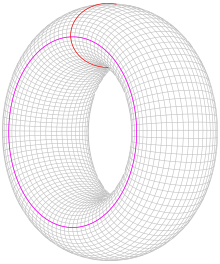
\includegraphics[scale=0.4]{tor.png}
            \caption{Tore de jeu$^1$}
            \label{fig:tore_de_jeu}
        \end{figure}
        
        Par défaut, nous avons implémenté des relations entre cases de type hexagonal (Figure \textbf{\ref{fig:pavage_hexagonal}}), comme il nous l'était imposé en début de projet. Cependant, dans le cadre d'un achievement nous avons également implémenté des changements de terrains qui impactent les relations faisant passer notre monde d'un pavage hexagonal, à un pavage carré (Figure \textbf{\ref{fig:pavage_carre}}) ou triagulaire (Figure \textbf{\ref{fig:pavage_triangulaire}}). Ces changements interviennent au bout d'un certain nombre de tour, nombre qui peut être paramétré par le joueur.
        
        \begin{figure}[H]
            \centering
            \begin{subfigure}{0.3\textwidth}
                \centering
                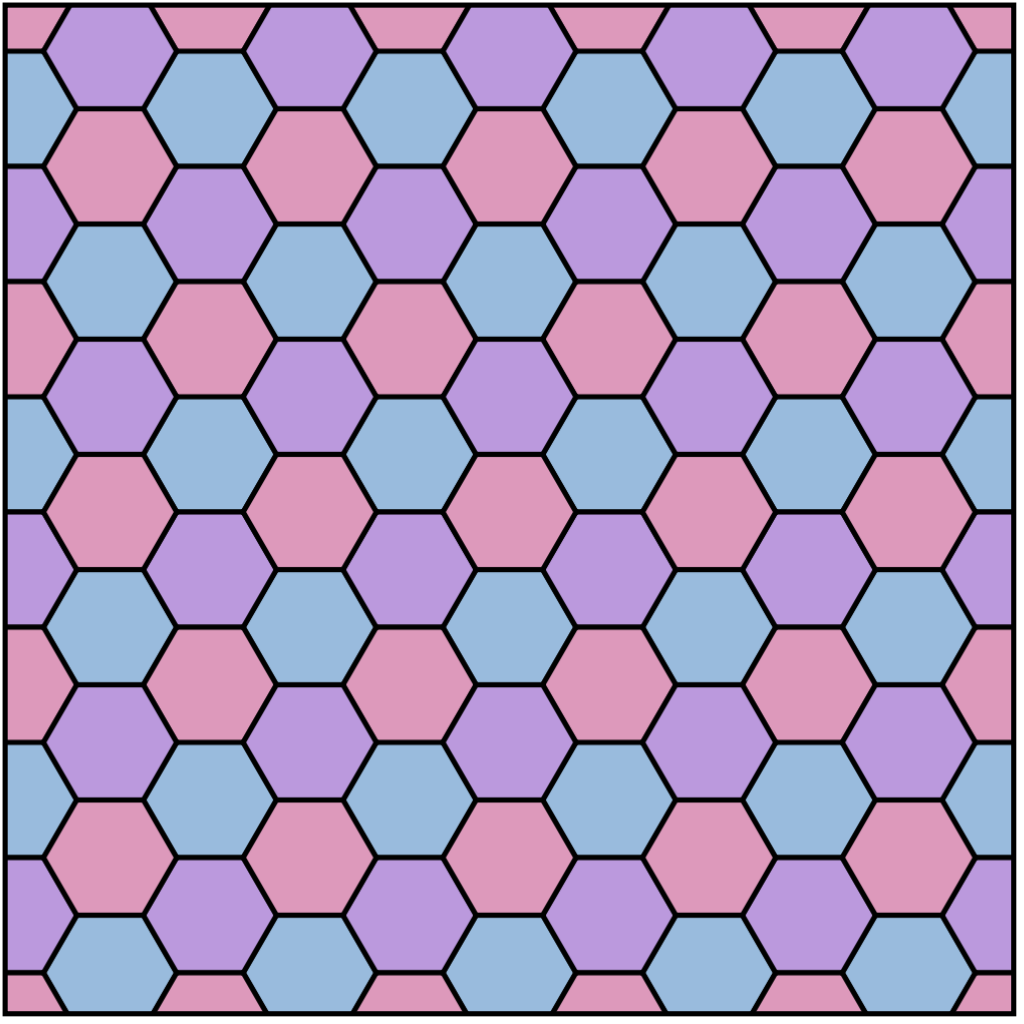
\includegraphics[width=\textwidth]{pavage_hexagonal.png}
                \caption{Pavage hexagonal\footnotemark[2]{}}
                \label{fig:pavage_hexagonal}
            \end{subfigure}
            \quad
            \begin{subfigure}{0.3\textwidth}
                \centering
                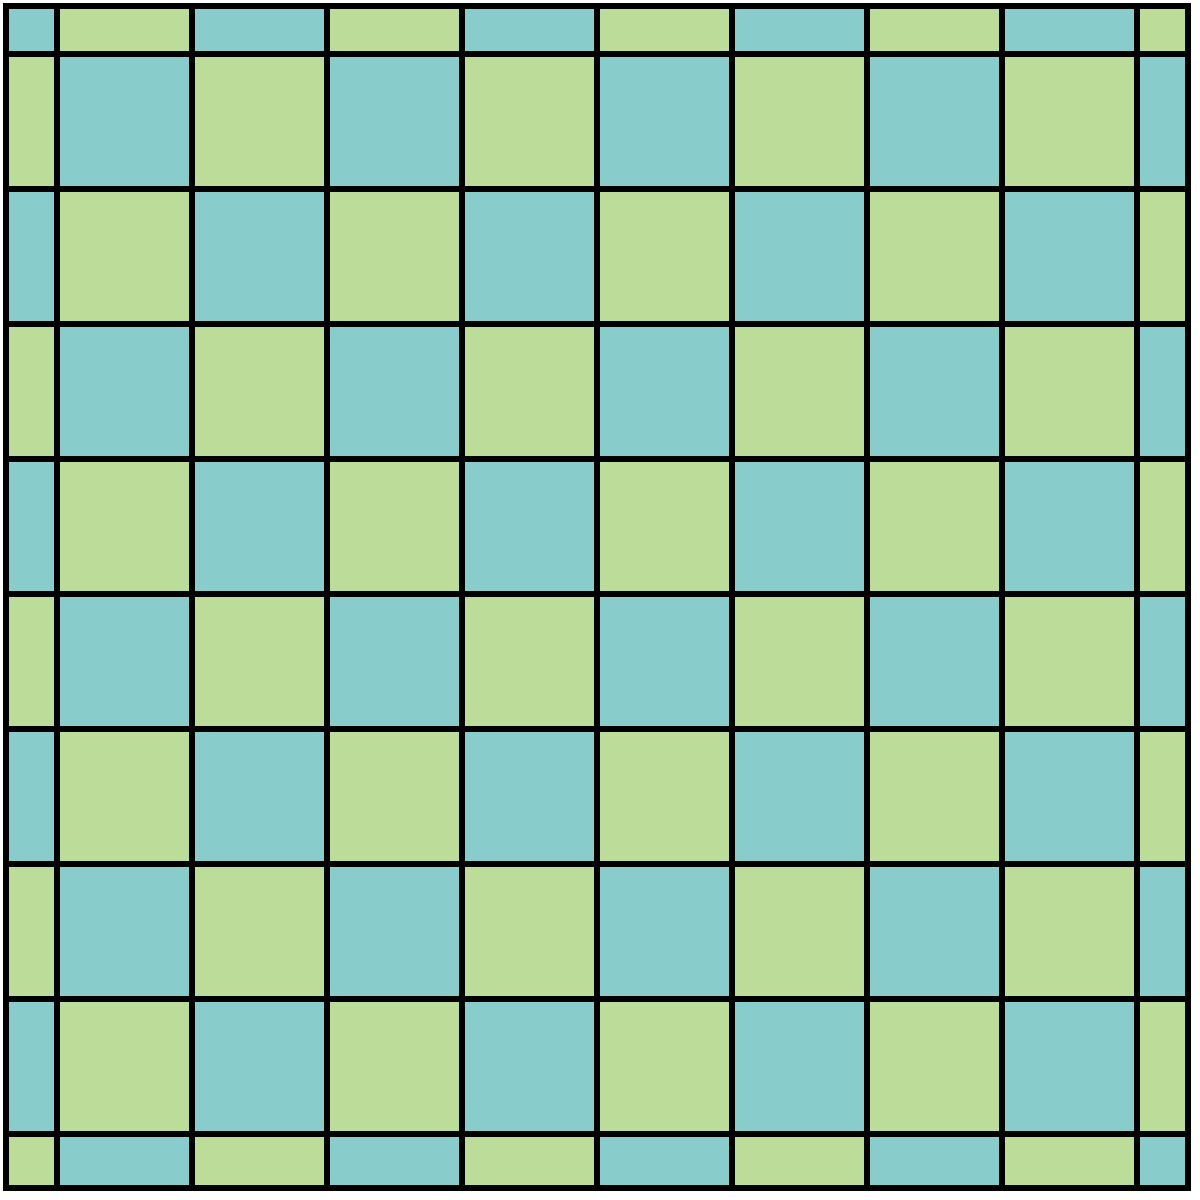
\includegraphics[width=\textwidth]{pavage_carre.png}
                \caption{Pavage carré\footnotemark[3]{}}
                \label{fig:pavage_carre}
            \end{subfigure}
            \quad 
            \begin{subfigure}{0.3\textwidth}
                \centering
                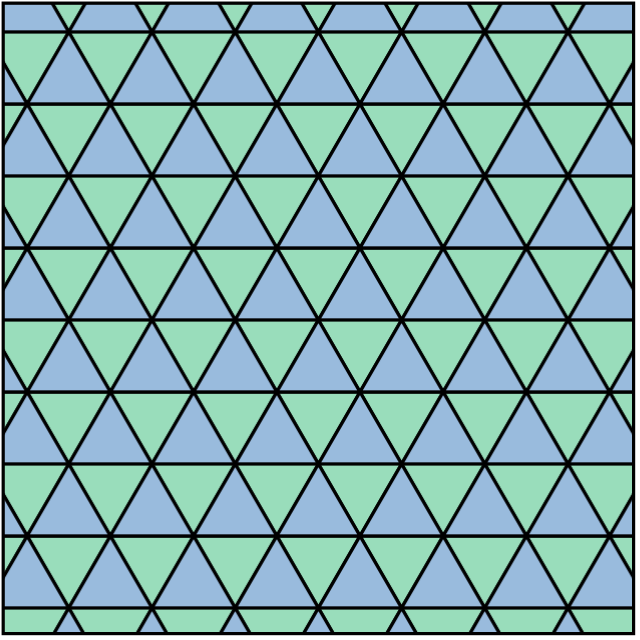
\includegraphics[width=\textwidth]{pavage_triangulaire.png}
                \caption{Pavage triangulaire\footnotemark[4]{}}
                \label{fig:pavage_triangulaire}
            \end{subfigure}
            \caption{Les différents pavages disponibles.}
            \label{label_de_la_figure 1}
        \end{figure}
        \footnotetext[1]{Source: \url{https://uk.wikipedia.org/wiki/\%D0\%9E\%D0\%B4\%D0\%BD\%D0\%BE\%D0\%B7\%D0\%B2'\%D1\%8F\%D0\%B7\%D0\%BD\%D0\%B0_\%D0\%BE\%D0\%B1\%D0\%BB\%D0\%B0\%D1\%81\%D1\%82\%D1\%8C}}
        \footnotetext[2]{Source: \url{https://fr.wikipedia.org/wiki/Pavage_hexagonal}}
        \footnotetext[3]{Source: \url{https://fr.wikipedia.org/wiki/Pavage_carr\%C3\%A9}}
        \footnotetext[4]{Source: \url{https://fr.wikipedia.org/wiki/Pavage_triangulaire}}

\section{Pièces et joueurs}
    \subsection{Pièces}\label{part:pawns}
        Premièrement, nous avons choisi d'implémenter de simples pions, pouvant se déplacer d'une seule case (seulement si celle-ci est vide), pour des raisons de facilité principalement. Par la suite, nous avons incorporé au jeu de nouvelles pièces, le rendant plus intéressant. Chaque pièce à un déplacement particulier. \\ 
        C'est pour cela que nous avons créé une structure qui rend les pièces modulables. Chaque pièce appartenant à cette structure est définie par un certain nombre d'arguments.
        \medbreak
        \begin{lstlisting}
/** A struct representing a piece */
struct pawns_t {
    int player_index;       // Numéro du joueur propriétaire du pion
    int max_dep;            // Nombres maximum de déplacements du pion
    enum color_t color;     // Couleur du pion
    enum sort_t type;       // Type du pion
    int position;           // Position du pion
    int captured;           // Etat du pion
};\end{lstlisting}

        \newpage
        
        \noindent Nous avons implémenté plusieurs types de piéces :
        \bigbreak

        
\includegraphics[width=0.45cm]{pawn.png} \textbf{Le Pion simpe :} \\
        Le pion est la pièce basique du jeu, il possède un seul mouvement dans la direction de son choix. Cependant il est possible d'en faire une dame d'échec en augmentant simplement son nombre de mouvements maximum afin qu'il puisse se déplacer sur de plus grandes distances.
        \medbreak
         \begin{figure}[H]
            \centering
            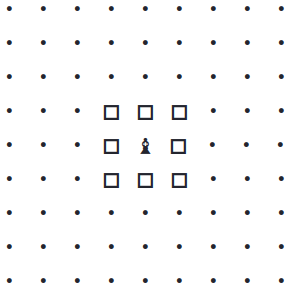
\includegraphics[scale=0.3]{img/dep_pawn.png}
            \caption{Déplacement d'un pion}
            \label{fig:dep_pawn}
        \end{figure}
            
        
\includegraphics[width=0.45cm]{tower.png} \textbf{La Tour :}\label{part:tower} \\
        Elle peut, comme aux échecs, se déplacer seulement en direction des points cardinaux. Nous avons décidé de limiter ses déplacements au Max(longueur du plateau, largeur du plateau). En effet, sans cette condition, étant donné l'apparence torique de notre plateau, ses movements pourraient être infinis.
        \medbreak
             \begin{figure}[H]
                \centering
                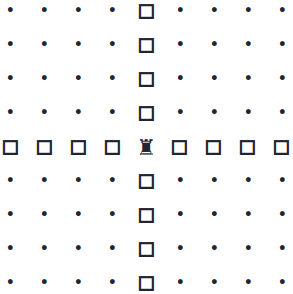
\includegraphics[scale=0.3]{img/dep_tower.png}
                \caption{Déplacement d'une tour}
                \label{fig:dep_tower}
            \end{figure}
        
\includegraphics[width=0.45cm]{elefun.png} \textbf{L'éléphant :} \\
        Il se déplace uniquement suivant les 4 directions cardinales, dans le cas de base, il dispose de deux déplacements successifs, mais cette valeur peut être modifiée.
        \medbreak
            \begin{figure}[H]
                \centering
                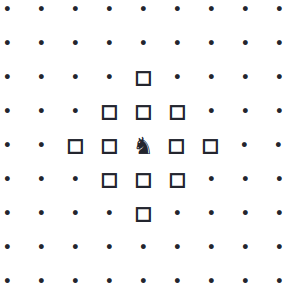
\includegraphics[scale=0.3]{img/dep_elefun.png}
                \caption{Déplacement de l'éléphant}
                \label{fig:dep_éléfun}
            \end{figure}
            
        
\includegraphics[width=0.45cm]{king.png} \textbf{Le Roi premier :} \\
        Il se téléporte directement sur les cases portant des numéros premiers.
        \medbreak
                     \begin{figure}[H]
                \centering
                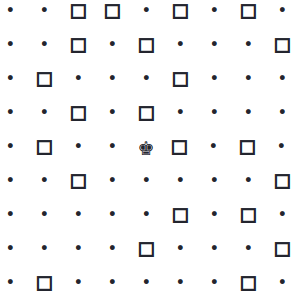
\includegraphics[scale=0.3]{img/dep_king.png}
                \caption{Déplacement du Roi}
                \label{fig:dep_king}
            \end{figure}
    
    \subsection{Joueurs}
        Un minimum de deux joueurs est nécessaire pour lancer une partie. Chaque joueur est associé à un index unique. Ils possèdent aussi une couleur, un nombre de pièces ainsi qu'un tableau qui les contient. La structure se présente comme ceci :
        \begin{lstlisting}
/** A struct representing a player */
struct players_t {
    int index;                          // Numéro du joueur 
    int pawns_nb;                       // Nombre de pièces
    struct pawns_t pawns[WORLD_SIZE/2]; // Tableau des pièces du joueur 
    enum color_t color;                 // Couleur du joueur
};\end{lstlisting}

        Le jeu peut également être joué à plus de deux joueurs en fonction de la taille du monde. L'implémentation de joueur tient à respecter l'équilibre du jeu. Donc si le plateau ne permet pas de répartir un certain nombre de joueurs différents à l'initialisation alors cet équilibre est rompu. 
    \subsection{Formations de départ}
            Pour plus de diversité, nous avons mis en place deux formations de départs différentes. Une première, classique, ressemblant aux échecs (mais toujours en prenant en considération la forme torique de notre plateau).
            \medbreak
            
            \begin{figure}[H]
                \centering
                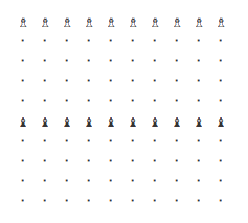
\includegraphics[scale=0.6]{departclassique.png}
                \caption{Départ classique}
                \label{fig:depart_classique}
            \end{figure}

            La deuxième formation que nous avons implémentée est plus particulière et présente le plateau sous forme de \textit{champs de bataille}, avec des énormes blocs de pièces séparés par des tranchées. Cette formation avait à l'origine pour but de tester la réaction des pièces lorsqu'elles sont entourées de pleins d'autres.
            \medbreak
            
            \begin{figure}[H]
                \centering
                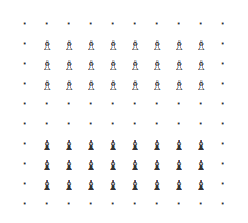
\includegraphics[scale=0.6]{img/battleground.png}
                \caption{Départ champ de bataille}
                \label{fig:depart_champ_de_bataille}
            \end{figure}

            Les types de pions qui composent ces formations sont modulables. Par défaut, la formation est remplie avec des pions simples. Néanmoins il est possible de changer cette pièce par défaut, ou encore d'ajouter un certain nombre de pièces "spéciales" en plus de la pièce par défaut. 
            
    \section{Boucle de jeu}

        \subsection{Sélection des options}
            Toujours dans le but d'augmenter la modularité de notre jeu, nous avons rendu un maximum d'options au choix du joueur lors de l'exécution. Les choix se font par l'intermédiaire de paramètres à ajouter lors de l'exécution du programme. Si les options sont écrites de manière incorrecte, le programme ne les prendra pas en compte et utilisera des valeurs par défaut.
            
        \subsection{Déroulement d'une partie}
            Lorsque le programme est lancé, le programme initialise un "monde extérieur", que nous verrons plus tard et qui contient le plateau de jeu, les joueurs et leurs pièces.
            \medbreak
            Au début de chaque tour, un contrôle sur le changement de terrain est effectué afin de le modifier (s'il est nécessaire, d'après les options de l'utilisateur). \\            Ensuite, une pièce du joueur est choisie au hasard pour se déplacer dans l'une des cases accessibles aléatoirement. Puis, on vérifie s'il y a un vainqueur ou si le max de tours a été atteint. Dans ce cas précis le jeu s'arrête et l'indique à l'utilisateur sinon on passe au tour suivant.
            
        \subsection{Conditions de victoire}
            Notre jeu admet deux conditions de victoire différentes :
            \begin{itemize}
                \item Le premier signe la fin du jeu dès lors qu'une pièce atteint les positions de départ de l'adversaire. Cette condition est dite "simple". Et permet de facilement vérifier les déplacements de nos pièces et le bon fonctionnement du jeu.
                \item La seconde nécessite que la totalité des pièces arrive dans les positions de départ de, ou des adversaires. Celle-ci est beaucoup plus complexe et nécessite des déplacements guidés pour l'atteindre. Cependant elle permet de faire durer plus longtemps les parties notamment en mode "champ de bataille" afin de voir beaucoup d'interactions. Cette condition est dite "complexe".
            \end{itemize}

\chapter{Architecture du projet}
\section{Relations}
    Notre jeu est basé sur les relations entre les différentes parties qui composent notre environnement de jeu.   
    \subsection{Voisinage}
        Le voisinage d'une pièce correspond aux places du monde qui sont dirrectement en contact avec la place de la pièce. Le nombre de voisins d'une pièce dépend donc de la géométrie de notre plateau (cf. \textbf{\ref{part:geometry}}). On va déterminer ces derniers en testant l'intégralité des directions disponibles pour la pièce en ne omettant pas de verifier si les cases sont occupées ou non. Cela nous donne donc un ensemble de cases disponibles pour cette dernière qui répond bien aux contraintes géométriques du plateau.
    \subsection{Déplacements}
        Nos déplacements sont réalisés en modifiant dans le monde l'état de la position ainsi que l'index associé à la pièce en question. Cela informe donc aux autres pièces que cette position est prise et permet de savoir à quel joueur elle appartient.
        \medbreak
        Pour determiner la position exacte du déplacement, on utilise un fonctionnement de recherche de proche en proche, qui va déterminer les voisins directs, puis en fonction du nombre de mouvements de la pièce, rééfectuer ce processus avec le voisin direct situé de la direction souhaitée. Le déplacement de cette dernière se fait ensuite aléatoirement parmi ces possibilités et comme dit précedemment, il est impossible pour cette dernière de choisir une case déjà occupée par une pièce alliée.
        \medbreak
        \noindent Dans le cas où toutes les cases sont occupées par une pièce alliée, le joueur ne peut pas jouer et son tour est passé.
        
    \subsection{Changements de terrain}
        Dès lors que la partie commence, une initialisation de la \textit{seed} du terrain est nécessaire. \newline
        Cette \textit{seed} influe directement sur les intéractions entre les différente position du monde et change donc les déplacements possibles. \\ Chaque pièce sera donc restrainte à un certain nombre de relations :
        
        \begin{itemize}
            \item Pour un terrain classique (hexagonal), toutes les directions sont autorisées.
            \item Pour un terrain à pavage triangulaire, une case sur deux possède les même relations de voisinage, on a ici les relations (N,SE,SW) pour une partie des pièces et (S,NE,NW) pour l'autre.
            \item Pour un terrain à pavage carré, les seules directions autorisées sont celles des points cardinaux (N,S,E,W).
        \end{itemize}
        \medbreak
        Après avoir réduit le nombre de directions possibles, le système de déplacement est appliqué de manière identique, elle prend alors compte des contraintes de direction. \newline
         \begin{figure}[H]
            \centering
            \begin{subfigure}{0.22\textwidth}
                \centering
                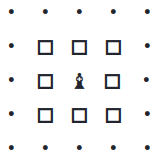
\includegraphics[scale= 0.35]{img/dep_hexagonal.png}
                \caption{Classique hexagonal}
                \label{fig:dep_hexa}
            \end{subfigure}
            \quad
            \begin{subfigure}{0.2\textwidth}
                \centering
                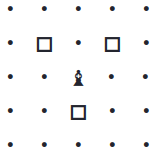
\includegraphics[scale= 0.35]{img/dep_triangle_1.png}
                \caption{Triangulaire 1}
                \label{fig:dep_tri1}
            \end{subfigure}
            \quad 
            \begin{subfigure}{0.2\textwidth}
                \centering
                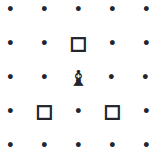
\includegraphics[scale= 0.35]{img/dep_triangle_2.png}
                \caption{ Triangulaire 2}
                \label{fig:de_triangulaire 2}
            \end{subfigure}
            \label{label_de_la_figure 3}
            \quad 
             \begin{subfigure}{0.2\textwidth}
                \centering
                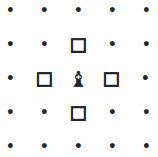
\includegraphics[scale= 0.35]{img/dep_carre.png}
                \caption{Carré}
                \label{fig:dep_carre}
            \end{subfigure}
            \caption{Les différents déplacements en fonction des pavages.}
        \end{figure}
        
        Nous avons donc réussi à implémenter un système qui en modifiant une \textit{seed} de terrain, modifie les relations de voisinage de la partie en cours.
    \subsection{Positions de départ}
        Etant donné l'aspect torique de notre plateau, nous avons dû faire très attention aux déséquilibres possibles en début de la partie, et ceci beaucoup plus que pour un plateau classique où il aurait suffit de positionner les pieces de chaque cotés de celui-ci.

        C'est pour résoudre ce problème que nous avons décidé d'utiliser un algorithme pour créer les formations en fonctions des paramètres. Pour cela, nous avons implémenté un algorithme qui en fonction des types de pièces à placer et de leur nombre, choisit une formation qui soit identique pour chaque joueur et qui ne crée pas de déséquilibre entre eux, et ceci quel que soit le nombre de joueurs ou la taille du plateau de jeu. Par exemple, la figure \textbf{\ref{fig:depart_classique_a_4}} montre les positions de départ pour une partie lancée avec 4 joueurs, sur un monde de taille $10\times10$, avec  $2$ tours (pièce, cf. \textbf{\ref{part:tower}}) par joueurs.
            
            \begin{figure}[H]
                \centering
                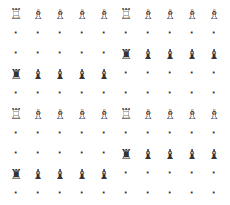
\includegraphics[scale=0.6]{img/depart_classique_a_4.png}
                \caption{Départ classique à 4}
                \label{fig:depart_classique_a_4}
            \end{figure}

        Cette facon de penser le départ du jeu nous a permis le rendre jeu encore plus modulable et de l'adapter à beaucoup plus de configurations en permettant des possibilités de départ presque infinies.
            
    \subsection{Capture et libération}
        Si une pièce atterit sur une pièce adverse, une capture est réalisée. Si la position de la pièce capturée est libre, elle a une probabilité d'être libérée. Cette probabilité est fixée à \texttt{50/100} mais peut être modifiée par l'utilisateur).
        La question de la capture d'une pièce adverse par un joueur est une des raisons qui nous ont poussé à créer un "monde extérieur" \texttt{world\_ext.c} (\textbf{cf. \ref{part:graph_src}}), qui sous forme d'une structre contient le plateau, les joueurs et les pions.
        \begin{lstlisting}
struct world_ext_t {
	struct world_t* world;                         // Plateau de jeu
	int nb_players;                                // Nombre de joueurs.
	struct players_t players[WORLD_SIZE];          // Liste des joueurs.
	struct sets_t initial_sets[WORLD_SIZE];        // Ensembles de positions de départ des joueurs.
	struct sets_t current_sets[WORLD_SIZE];        // Ensembles de positions prises par chaque joueurs.
	int nb_captured_pawns;                         // Nombre de pièces capturées.
	struct pawns_t* captured_pawns[WORLD_SIZE];    // Liste des pièces capturées.
};\end{lstlisting}
        \noindent L'implémentation de cette fonction nous a permis d'implémenter la capture de cette façon :
        \begin{itemize}
            \item Lorsqu'une pièce est capturée, sont attribut \texttt{captured} (cf. \textbf{\ref{part:pawns}}) prend la valeur \texttt{1}.
            \item La pièce est ajoutée à la liste des pièces capturées : \texttt{captured\_pawns[]}, et sa position est retirée de la liste des positions prises par le joueur : \texttt{current\_sets[index\_du\_joueur][]}.
        \end{itemize}
        \medbreak
        Procéder de cette manière nous a permis de ne pas modifier la position de la pièce capturée, ainsi, elle la garde en mémoire. Lorsque les conditions de libération sont remplies, on effectue le schéma inverse, et la pièce est de retour sur le plateau. 

\section{Inclusions et organisation du projet (Makefile?)}

    \subsection{Organisation du monde}
    \subsection{Dépendances des fichiers}\label{part:graph_src}
        Afin de rendre le projet le plus modulable possible, nous avons séparé notre projet en plusieurs fichiers \texttt{.c}, ces fichiers contienent les fonctions qui permettent au tout de fonctionner. Chacun de ces fichiers \texttt{.c} inclu un fichier \texttt{.h} du même nom. Ces fichiers d'entête contiennent les \texttt{header} de toutes les fonctions "publiques" qui ont pour but d'être utilisées par d'autres fichiers. Les inclusions ne se font jamais entre les fichiers \texttt{.c}, mais uniquement avec les \texttt{.h}.
        
        \begin{figure}[H]
            \centering
            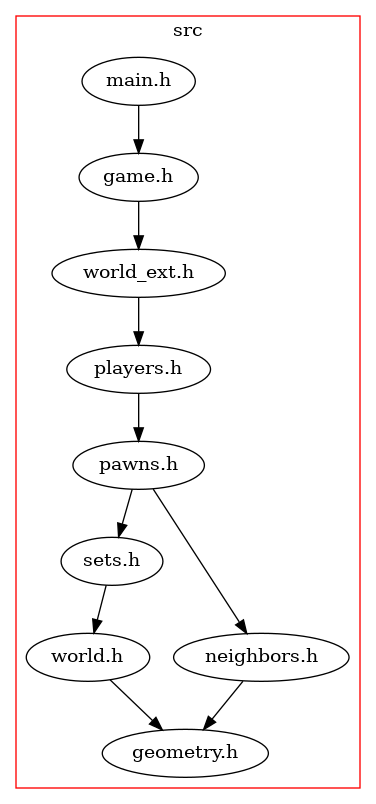
\includegraphics[scale=0.4]{img/graph_src.png}
            \caption{Graphique de dépendance des fichiers source. \textit{Généré avec} \texttt{Graphviz}.}
            \label{fig:graph_src}
        \end{figure}

        Cette organisation du projet à base d'inclusions nous permet une très grande modularité. En effet, si un fichier \texttt{.c} est modifié (comme par exemple \texttt{world.c}), le projet continue de fonctionner tant que la nouvelle implémentation respecte le fichier \texttt{.h} correspondant.

    \subsection{Compilation}
        Pour faciliter les travaux de compilations séparés, nous avons intégré un fichier \texttt{Makefile}. Ce fichier nous a permis de déclarer des règles générales qui simplifient les commandes de compilations. Nous nous en somme par exemple servi pour compiler automatiquement tous les fichiers \texttt{.o} nécessaires, ou encore pour compiler et éxécuter tous les tests en même temps.

\section{Tests}
    \subsection{Structure des tests}
        Nous avons décidé de séparer les tests dans différents fichiers pour plus de flexibilité. Chaque fichier test contient les fonctions visants à tester un unique fichier source. Cette méthode nous a permis de pouvoir tester l'ensemble du code source en même temps, ou bien de lancer les tests d'un fichier en particulier.

        \begin{figure}[H]
            \centering
            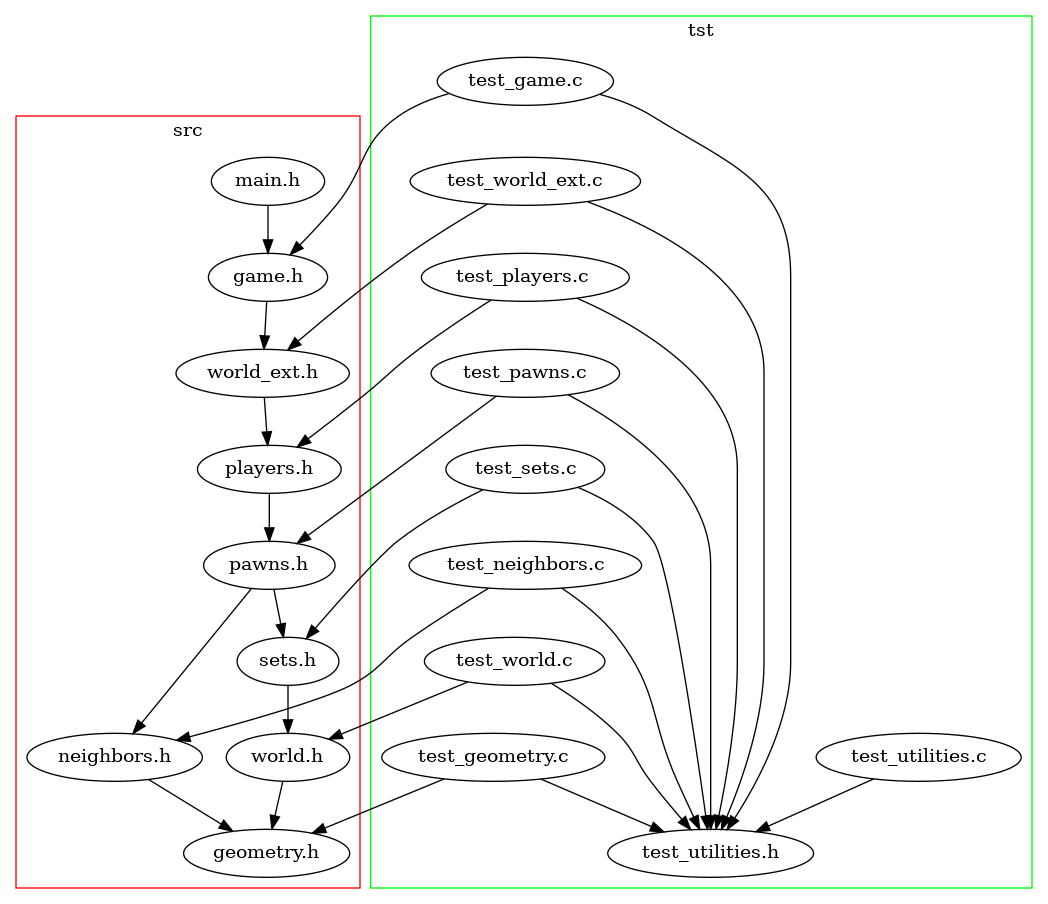
\includegraphics[scale=0.4]{img/graph_tst.png}
            \caption{Graphique de dépendance des fichiers tests. \textit{Généré avec} \texttt{Graphviz}.}
            \label{fig:graph_tst}
        \end{figure}

        La figure \textbf{\ref{fig:graph_tst}} montre les inclusions de nos fichiers tests. On remarque que chaque fichier test inclu uniquement le fichier source qu'il teste. De plus, nous avons décidés de séparer deux fonctions générales des tests dans un fichier \texttt{test\_utilities.c}. Ce fichier est le seul des fichiers tests à avoir un fichier d'entête, car c'est le seul qui est inclu dans d'autres fichiers. Il contient les deux fonctions suivantes :
        
        \begin{lstlisting}
void str_test(const char str1[], const char str2[]) // Compare 2 strings
{ 
    (!strcmp(str1, str2)) ? printf("\t\tPASSED\n") : printf("\t\tRecieve %s instead of %s.\n", str1, str2);
}

void int_test(const int int1, const int int2) // Compare 2 integers
{
    (int1 == int2) ? printf("\t\tPASSED\n") : printf("\t\tRecieve %d instead of %d.\n", int1, int2);
}\end{lstlisting}

        Ces deux fonctions nous ont été très utiles dans le cadre de la \textbf{programmation par le test}. En effet, appeler celles-ci dans nos fichiers tests nous a permis de très facilement comparer les retours des fonctions testées avec ce que nous attendions. En cas de réussite, le programme affiche : \texttt{PASSED}, tandis que si le test ne passe pas, le programme affichera : \texttt{Recieve <valeur\_reçu> instead of <valeur\_attendue>}.
        \medbreak
        Nous avons donc pu écrire nos tests, puis implémenter nos fonctions jusqu'à ce que tous nos tests affichent : \texttt{PASSED}.
        

        
    

\chapter{Conclusion}

\section{Difficultés rencontrées}

\section{Points à améliorer}

\section{Ce que le projet nous a apporté}

%==================================================%

\begin{itemize}
    \item Environement de jeu (variable pions etc)
    \begin{itemize}
        \item Structure et Variables globales:
        
        \item Plateau :



        \item Pieces :
        \\
               
        \item Joueurs

        Les joueurs sont définis par une structure qui contient un certain nombre d'élément:
        \begin{itemize}
            \item Un index qui diférencies les joueurs entre eux
            \item Le nombre de pion qu'il possède
            \item Le nombre de ses pions capturés
            \item Une liste de ses pions
            \item Une couleur
        \end{itemize}
        \item Boucle de jeu
        \begin{itemize}
            \item Déroulement de la partie 
            \item Conditions de victoire
        \end{itemize}
    \end{itemize}

    
    \item Architecture 
    \begin{itemize}
        \item Relation de jeu 
        \begin{itemize}
            \item Relations de voisinage 
            \item Relation d'initialisation de partie 
            \item Interation entre les joueurs (prisons)
            \item Interaction entre le monde et les joueurs 
        \end{itemize}
        \item Inclusion
        \begin{itemize}
            \item Makefile
            \item Organisation des fichiers projets
            \item Organisation des fichiers de test
        \end{itemize}
        \item Complexité 
    \end{itemize}
    \item Tests 
    \begin{itemize}
        \item Structures Tests
        \item Notre utilisation des tests pour le bon focntionnement du projet 
    \end{itemize}
    \item Difficultées rencontrées 
    \begin{itemize}
        \item Problème de structure
        \item Difficulté d'affichage  
        \item Aléatoire 
    \end{itemize}
    \end{itemize}

Conclusion
\begin{itemize}
    \item Points à amélioré
    \begin{itemize}
        \item Les test
        \item Travailler l'indépendance 
        
    \end{itemize}
    \item Ce que le projet nous a apporté 
    \begin{itemize}
        \item Découverte de GitHub
        \item Découverte du Makefile
        \item Progression en C
        
    \end{itemize}
\end{itemize}


\end{document}
